\section{The unique hierarchy}\label{sec:hierarchy}

% ledger: R4-R8, T8, T9, N1, N2, E4; source PROOFS_registered.md R§7-R§9; ruling R7 (MECHANIZATION_PLAN.md C3); Lean first_shells_33, central_completion, parent_conflicts_28 (T1n), parent_local_to_global, carrier_hierarchy, carrier_hierarchy_unique (spine)
From now on every tiling is registered (\cref{thm:registration}), and the argument is finite
combinatorics on the lattice plus one scale argument. For each of the eight children of
\cref{tab:children} there is one candidate parent through a root chair in the identity pose:
apply the inverse child pose to the list of children. Each candidate is a cluster of eight chairs
whose baseline is a congruent copy of $2\carrier$.

\begin{lemma}[first shells; R\S7, \tier{T1n} \lean{first\_shells\_33}]\label[lemma]{lem:shells}
There are exactly $33$ ways to cover the $22$ shell cells of a root chair by legal neighbours
from $\atlas$ without overlaps and without an illegal contact between chosen neighbours. Each of
the $33$ contains the face-adjacent sibling signature of exactly one candidate parent.
\end{lemma}

The $33$ arrangements (\cref{fig:shells}) are necessary local configurations, not claims that each extends to a
tiling; a second implementation, using a set-based recursion instead of the generator's bitmask
recursion, reproduces all $33$.

% ledger: R5; Lean central_completion (T1n)
\begin{lemma}[central completion; R\S7, \tier{T1n} \lean{central\_completion}]\label[lemma]{lem:central}
In one of the $33$ arrangements the root is the central child of its proposed parent and all
seven outer children are present. In the other $32$ the proposed parent's centre is a neighbour of
the root; checking every first shell at that centre for compatibility with the arrangement, $18$
of the $32$ have no compatible completion and cannot occur in a tiling, $14$ have completions,
and every completion makes the proposed centre genuinely central.
\end{lemma}

\begin{lemma}[parent conflicts; R\S7, \tier{T1n} \lean{parent\_conflicts\_28}]\label[lemma]{lem:conflicts}
Each of the $28$ unordered pairs of distinct candidate parents through one root contains an
incompatible pair of child poses.
\end{lemma}

\begin{theorem}[unique parent; R\S7 Theorem 7.1; \lean{parent\_local\_to\_global},
\lean{unique\_parent}: \tier{T1n}, unconditional]\label{thm:parent}
Every tiling by $\solid$ partitions uniquely into the eight-chair parent clusters, and the
parent of each tile is determined by a finite neighbourhood of it.
\end{theorem}

\begin{proof}
Registration gives the complete local inventory around a tile: its first shell is one of the $33$
of \cref{lem:shells}, which proposes a unique parent. By \cref{lem:central} that parent's seven
other children are present in every tiling in which the shell occurs. By \cref{lem:conflicts}
two parents cannot share a tile, so the local assignments are globally disjoint and consistent,
and every tile is included.
\end{proof}

\begin{figure}[ht]
  \centering
  {\scriptsize% generated by paper/scripts/first_shells.py from certificates/candidate_certificate.json
\begin{tabular}{rlll}
\toprule
shell & atlas contacts & parent & completion \\
\midrule
1 & 3,9,10,12,20,29,38,40 & 7 & central \\
2 & 10,13,16,18,21,22,41 & 0 & completable \\
3 & 1,9,10,13,22,27,37,41 & 0 & completable \\
4 & 2,4,11,16,18,21,42 & 6 & completable \\
5 & 4,11,14,16,18,21,42 & 6 & impossible \\
6 & 11,14,15,16,18,21,42 & 2 & completable \\
7 & 4,11,16,18,21,22,42 & 6 & impossible \\
8 & 11,16,18,21,22,23,42 & 1 & completable \\
9 & 11,14,16,18,21,26,42 & 3 & impossible \\
10 & 11,16,18,21,22,26,42 & 3 & impossible \\
11 & 11,16,18,21,25,26,42 & 3 & completable \\
12 & 11,14,16,18,21,34,42 & 5 & impossible \\
13 & 11,16,18,21,22,34,42 & 5 & impossible \\
14 & 11,16,18,21,33,34,42 & 5 & completable \\
15 & 1,2,4,9,11,27,37,42 & 6 & completable \\
16 & 1,4,9,11,14,27,37,42 & 6 & impossible \\
17 & 1,9,11,14,15,27,37,42 & 2 & completable \\
\bottomrule
\end{tabular}
\par\smallskip
\begin{tabular}{rlll}
\toprule
shell & atlas contacts & parent & completion \\
\midrule
18 & 1,4,9,11,22,27,37,42 & 6 & impossible \\
19 & 1,9,11,22,23,27,37,42 & 1 & completable \\
20 & 1,9,11,14,26,27,37,42 & 3 & impossible \\
21 & 1,9,11,22,26,27,37,42 & 3 & impossible \\
22 & 1,9,11,25,26,27,37,42 & 3 & completable \\
23 & 1,9,11,14,27,34,37,42 & 5 & impossible \\
24 & 1,9,11,22,27,34,37,42 & 5 & impossible \\
25 & 1,9,11,27,33,34,37,42 & 5 & completable \\
26 & 4,11,16,18,21,42,43 & 6 & impossible \\
27 & 11,16,18,21,26,42,43 & 3 & impossible \\
28 & 11,16,18,21,34,42,43 & 5 & impossible \\
29 & 1,4,9,11,27,37,42,43 & 6 & impossible \\
30 & 1,9,11,26,27,37,42,43 & 3 & impossible \\
31 & 1,9,11,27,34,37,42,43 & 5 & impossible \\
32 & 11,16,18,21,42,43,44 & 4 & completable \\
33 & 1,9,11,27,37,42,43,44 & 4 & completable \\
\bottomrule
\end{tabular}
}
  \caption{The $33$ first shells, their proposed parent types and central-completion outcomes.}
  \label{fig:shells}
\end{figure}

% ledger: R7, E4; Lean parent_atlas_eq_fine (T1n), parent_atlas_admissibility, parent_common_parity, halved_parent_baseline_tiling (spine); small_collar_realization_holds (T1n)
\begin{theorem}[admissibility-preserving coarsening; R\S8 Theorem 8.1; \tier{T1n},
unconditional]\label{thm:coarsening}
Let $D$ group a tiling $T$ into its unique parents, divide the parent origins and the scale by
two, and replace each parent's baseline by a fresh copy of $\solid$ in that frame. Then $D(T)$ is
again a tiling by $\solid$, and $D(T+v)=D(T)+v/2$ for every vector $v$.
\end{theorem}

In Lean the two clauses are \lean{coarsening\_is\_tiling} and
\lean{coarsening\_translation\_equivariant}; the physical realization of the coarsened tiling
uses the theorem \lean{small\_collar\_realization\_holds} (\tier{T1n}, \cref{sec:existence}) and
the tube construction.

\begin{proof}
The parent bodies partition space and their contact graph is connected, since the unit-cell
adjacency graph is. Every contact between two parents is one of the $44$ legal parent contacts
of \cref{sec:designtest}, whose translations are all even, so all parent origins lie in one coset
of $2\Z^3$ and halving puts them on a common lattice; by the identity of \cref{sec:designtest}
every halved contact belongs to $\atlas$. The halved baseline tiling is therefore a registered
chair tiling whose profiles match on every shared panel, and the small-collar realization lemma
(\cref{sec:existence}) turns it into a tiling by $\solid$. Translation covariance holds because
the parents of $T+v$ are the parents of $T$ translated by $v$ (\cref{thm:parent}), and the
origins are then divided by two; no phase is chosen, the actual parent origins are used.
\end{proof}

% ledger: R11 (E4)
The coset of $2\Z^3$ may be $(1,1,1)+2\Z^3$, so that $D(T)$ sits on a half-integer coset after
halving; periods are differences of poses within one coset and remain integer vectors, which
is all \cref{sec:aperiodicity} uses. $D$ is not a homothety of each cluster's corrugated surface
into $\solid$: it decodes the carrier and re-standardizes the surface by the same admissible
rule, which is why an exact self-similar corrugated macro-shape is not needed.

% ledger: T8, T9, N1, N2, R8; ruling R7; Lean carrier_hierarchy, carrier_hierarchy_unique, geometric_hierarchy_canonical, geometric_hierarchy_unique, nested_substitution_controls, hierarchy_cell_controls (T1n)
Iterating $D$ gives the hierarchy. Call a \emph{supertile of level $n$} a $2^n$-scaled chair in
a registered pose, and say that a family of partitions of the registered cells of $T$ into
level-$n$ supertiles, one partition for each $n$, is \emph{nested} if every level-$(n+1)$
supertile is exactly the union of its eight geometric child supertiles at level $n$.

\begin{theorem}[the intrinsic hierarchy; ruling R7; \tier{T1n}, unconditional:
\lean{carrier\_hierarchy}, \lean{carrier\_hierarchy\_unique},
\lean{geometric\_hierarchy\_canonical}, \lean{geometric\_hierarchy\_unique}]\label{thm:hierarchy}
Every tiling $T$ by $\solid$ carries a nested family of partitions into supertiles of every level,
with level $0$ the registered carrier tiling associated with $T$, and any two nested families
coincide level by level.
\end{theorem}

\begin{proof}
Existence: the level-$n$ partition is read off $D^n(T)$, each level-$n$ supertile being a chair
of $D^n(T)$ scaled by $2^n$ back to the coordinates of $T$; nesting is the definition of $D$.
Uniqueness: a nested family's level-$(n+1)$ partition is a partition of the level-$n$ supertiles
into parents, which \cref{thm:parent} applied to $D^n(T)$ determines; induct on $n$.
\end{proof}

% ledger: T8, M9 (closed); external review of the manuscript 2026-09-09, finding M2; pinned LogicalSpine.lean (LevelSupertilePose, carrier_hierarchy_unique, GeometricHierarchy, geometric_hierarchy_canonical, geometric_hierarchy_unique, carrierHierarchy_geometric); negative/NoncanonicalGeometricHierarchy.lean
The pinned Lean declarations prove this in two steps. \lean{carrier\_hierarchy\_unique} is stated
in the type whose level-$n$ poses belong to $D^n(T)$ (the structure \lean{LevelSupertilePose}
carries that membership). The structure \lean{GeometricHierarchy} carries no such membership: its
data are the raw poses, each level registered by one common rigid motion, with the nesting law of
the theorem; \lean{geometric\_hierarchy\_canonical} proves, by induction on the level from the
unique-parent theorem, that every pose of such a family lies in $D^n(T)$, and
\lean{geometric\_hierarchy\_unique} then gives uniqueness among arbitrary geometrically nested
registered families, \lean{carrierHierarchy\_geometric} supplying the existence half in the raw
type. The written induction above is the content of the first of these theorems. The raw
structure has no canonicity-membership field. The must-fail control
(\file{negative/NoncanonicalGeometricHierarchy.lean}) attempts to prove that a level-one pose is
noncanonical using \lean{geometric\_hierarchy\_canonical}; it checks that the positive membership
proof is rejected at the negated type.

% ledger: T9, N1, N2, L10; source SMKGS24 (fault lines); paper/scripts/seed_language_closure.py (T2); external review of the manuscript 2026-09-09, finding M1
Two things are deliberately not claimed. The theorem has no exhaustion clause: it does not say
that the supertiles containing one fixed tile grow to cover space, and they need not. The
substitution fixed point with seed $(6,0,4,5,2,3,0,1)$ (\cref{sec:limitperiodic}) has near the
origin two whole tiles in the frame $A=\operatorname{diag}(-1,-1,1)$, at the origin and at
$(1,1,-1)$; the first is its own child $000$ at every level, so its ancestors are the supertiles
$2^nA\carrier$, whose union is the closed octant $\{x\le0,\ y\le0,\ z\ge0\}$ and not all of
space, and the second is its own central child, its ancestors filling the closure of the
complement. This is a tiling with an infinite fault surface on supertile boundaries at all
levels, of the kind the hat paper contemplates for hats: ``it is conceivable that [tiles] could
tile infinite sectors of the plane, which could then be combined into tilings with infinite
`fault lines' that lie on the boundaries of supertiles at all levels'' \cite{SMKGS24}. It is
nevertheless substitution-legal, every finite patch of it occurring inside a supertile, so
non-exhaustion does not by itself take a tiling out of the substitution hull; whether every
tiling by $\solid$ lies in that hull is a separate question, left open (\cref{sec:remarks}).
Nor is the hierarchy claimed to
be locally derivable from the tiling by unmarked chairs: an unmarked chair has eight proper
orientations while a registered pose of $\solid$ is one of $24$, so the frame of a chair carries
a $\Z/3$ of information invisible to its geometry, and the parent is read from the features,
not from the chairs. What the theorem gives is exactly what \cref{sec:aperiodicity} needs: a
grouping at every scale that the tiling determines and that every symmetry of the tiling
therefore preserves. The same-frame grandchild at $(2,2,2)$ and the first two nested patches
($64$ and $4{,}096$ tiles, $448$ and $28{,}672$ cells) are checked in Lean as controls
(\cref{fig:nesting}).

\begin{figure}[ht]
  \centering
  \resizebox{0.8\linewidth}{!}{% generated by paper/scripts/nesting_slice.py from certificates/candidate_certificate.json (children)
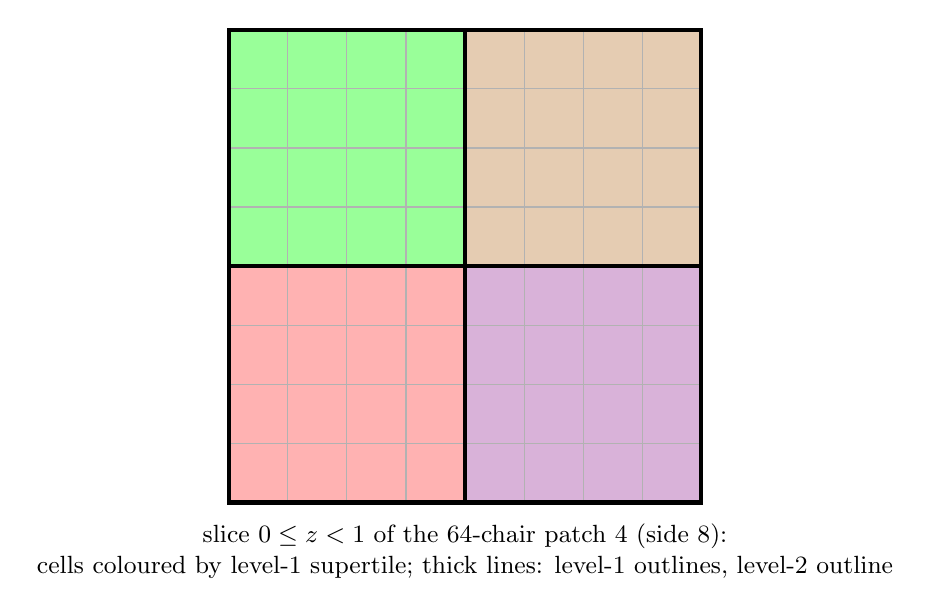
\begin{tikzpicture}[x=1cm,y=1cm,font=\scriptsize]
  \fill[red!30] (0.0,0.0) rectangle (0.75,0.75);
  \draw[gray!60,thin] (0.0,0.0) rectangle (0.75,0.75);
  \fill[red!30] (0.0,0.75) rectangle (0.75,1.5);
  \draw[gray!60,thin] (0.0,0.75) rectangle (0.75,1.5);
  \fill[red!30] (0.0,1.5) rectangle (0.75,2.25);
  \draw[gray!60,thin] (0.0,1.5) rectangle (0.75,2.25);
  \fill[red!30] (0.0,2.25) rectangle (0.75,3.0);
  \draw[gray!60,thin] (0.0,2.25) rectangle (0.75,3.0);
  \fill[green!40] (0.0,3.0) rectangle (0.75,3.75);
  \draw[gray!60,thin] (0.0,3.0) rectangle (0.75,3.75);
  \fill[green!40] (0.0,3.75) rectangle (0.75,4.5);
  \draw[gray!60,thin] (0.0,3.75) rectangle (0.75,4.5);
  \fill[green!40] (0.0,4.5) rectangle (0.75,5.25);
  \draw[gray!60,thin] (0.0,4.5) rectangle (0.75,5.25);
  \fill[green!40] (0.0,5.25) rectangle (0.75,6.0);
  \draw[gray!60,thin] (0.0,5.25) rectangle (0.75,6.0);
  \fill[red!30] (0.75,0.0) rectangle (1.5,0.75);
  \draw[gray!60,thin] (0.75,0.0) rectangle (1.5,0.75);
  \fill[red!30] (0.75,0.75) rectangle (1.5,1.5);
  \draw[gray!60,thin] (0.75,0.75) rectangle (1.5,1.5);
  \fill[red!30] (0.75,1.5) rectangle (1.5,2.25);
  \draw[gray!60,thin] (0.75,1.5) rectangle (1.5,2.25);
  \fill[red!30] (0.75,2.25) rectangle (1.5,3.0);
  \draw[gray!60,thin] (0.75,2.25) rectangle (1.5,3.0);
  \fill[green!40] (0.75,3.0) rectangle (1.5,3.75);
  \draw[gray!60,thin] (0.75,3.0) rectangle (1.5,3.75);
  \fill[green!40] (0.75,3.75) rectangle (1.5,4.5);
  \draw[gray!60,thin] (0.75,3.75) rectangle (1.5,4.5);
  \fill[green!40] (0.75,4.5) rectangle (1.5,5.25);
  \draw[gray!60,thin] (0.75,4.5) rectangle (1.5,5.25);
  \fill[green!40] (0.75,5.25) rectangle (1.5,6.0);
  \draw[gray!60,thin] (0.75,5.25) rectangle (1.5,6.0);
  \fill[red!30] (1.5,0.0) rectangle (2.25,0.75);
  \draw[gray!60,thin] (1.5,0.0) rectangle (2.25,0.75);
  \fill[red!30] (1.5,0.75) rectangle (2.25,1.5);
  \draw[gray!60,thin] (1.5,0.75) rectangle (2.25,1.5);
  \fill[red!30] (1.5,1.5) rectangle (2.25,2.25);
  \draw[gray!60,thin] (1.5,1.5) rectangle (2.25,2.25);
  \fill[red!30] (1.5,2.25) rectangle (2.25,3.0);
  \draw[gray!60,thin] (1.5,2.25) rectangle (2.25,3.0);
  \fill[green!40] (1.5,3.0) rectangle (2.25,3.75);
  \draw[gray!60,thin] (1.5,3.0) rectangle (2.25,3.75);
  \fill[green!40] (1.5,3.75) rectangle (2.25,4.5);
  \draw[gray!60,thin] (1.5,3.75) rectangle (2.25,4.5);
  \fill[green!40] (1.5,4.5) rectangle (2.25,5.25);
  \draw[gray!60,thin] (1.5,4.5) rectangle (2.25,5.25);
  \fill[green!40] (1.5,5.25) rectangle (2.25,6.0);
  \draw[gray!60,thin] (1.5,5.25) rectangle (2.25,6.0);
  \fill[red!30] (2.25,0.0) rectangle (3.0,0.75);
  \draw[gray!60,thin] (2.25,0.0) rectangle (3.0,0.75);
  \fill[red!30] (2.25,0.75) rectangle (3.0,1.5);
  \draw[gray!60,thin] (2.25,0.75) rectangle (3.0,1.5);
  \fill[red!30] (2.25,1.5) rectangle (3.0,2.25);
  \draw[gray!60,thin] (2.25,1.5) rectangle (3.0,2.25);
  \fill[red!30] (2.25,2.25) rectangle (3.0,3.0);
  \draw[gray!60,thin] (2.25,2.25) rectangle (3.0,3.0);
  \fill[green!40] (2.25,3.0) rectangle (3.0,3.75);
  \draw[gray!60,thin] (2.25,3.0) rectangle (3.0,3.75);
  \fill[green!40] (2.25,3.75) rectangle (3.0,4.5);
  \draw[gray!60,thin] (2.25,3.75) rectangle (3.0,4.5);
  \fill[green!40] (2.25,4.5) rectangle (3.0,5.25);
  \draw[gray!60,thin] (2.25,4.5) rectangle (3.0,5.25);
  \fill[green!40] (2.25,5.25) rectangle (3.0,6.0);
  \draw[gray!60,thin] (2.25,5.25) rectangle (3.0,6.0);
  \fill[violet!30] (3.0,0.0) rectangle (3.75,0.75);
  \draw[gray!60,thin] (3.0,0.0) rectangle (3.75,0.75);
  \fill[violet!30] (3.0,0.75) rectangle (3.75,1.5);
  \draw[gray!60,thin] (3.0,0.75) rectangle (3.75,1.5);
  \fill[violet!30] (3.0,1.5) rectangle (3.75,2.25);
  \draw[gray!60,thin] (3.0,1.5) rectangle (3.75,2.25);
  \fill[violet!30] (3.0,2.25) rectangle (3.75,3.0);
  \draw[gray!60,thin] (3.0,2.25) rectangle (3.75,3.0);
  \fill[brown!40] (3.0,3.0) rectangle (3.75,3.75);
  \draw[gray!60,thin] (3.0,3.0) rectangle (3.75,3.75);
  \fill[brown!40] (3.0,3.75) rectangle (3.75,4.5);
  \draw[gray!60,thin] (3.0,3.75) rectangle (3.75,4.5);
  \fill[brown!40] (3.0,4.5) rectangle (3.75,5.25);
  \draw[gray!60,thin] (3.0,4.5) rectangle (3.75,5.25);
  \fill[brown!40] (3.0,5.25) rectangle (3.75,6.0);
  \draw[gray!60,thin] (3.0,5.25) rectangle (3.75,6.0);
  \fill[violet!30] (3.75,0.0) rectangle (4.5,0.75);
  \draw[gray!60,thin] (3.75,0.0) rectangle (4.5,0.75);
  \fill[violet!30] (3.75,0.75) rectangle (4.5,1.5);
  \draw[gray!60,thin] (3.75,0.75) rectangle (4.5,1.5);
  \fill[violet!30] (3.75,1.5) rectangle (4.5,2.25);
  \draw[gray!60,thin] (3.75,1.5) rectangle (4.5,2.25);
  \fill[violet!30] (3.75,2.25) rectangle (4.5,3.0);
  \draw[gray!60,thin] (3.75,2.25) rectangle (4.5,3.0);
  \fill[brown!40] (3.75,3.0) rectangle (4.5,3.75);
  \draw[gray!60,thin] (3.75,3.0) rectangle (4.5,3.75);
  \fill[brown!40] (3.75,3.75) rectangle (4.5,4.5);
  \draw[gray!60,thin] (3.75,3.75) rectangle (4.5,4.5);
  \fill[brown!40] (3.75,4.5) rectangle (4.5,5.25);
  \draw[gray!60,thin] (3.75,4.5) rectangle (4.5,5.25);
  \fill[brown!40] (3.75,5.25) rectangle (4.5,6.0);
  \draw[gray!60,thin] (3.75,5.25) rectangle (4.5,6.0);
  \fill[violet!30] (4.5,0.0) rectangle (5.25,0.75);
  \draw[gray!60,thin] (4.5,0.0) rectangle (5.25,0.75);
  \fill[violet!30] (4.5,0.75) rectangle (5.25,1.5);
  \draw[gray!60,thin] (4.5,0.75) rectangle (5.25,1.5);
  \fill[violet!30] (4.5,1.5) rectangle (5.25,2.25);
  \draw[gray!60,thin] (4.5,1.5) rectangle (5.25,2.25);
  \fill[violet!30] (4.5,2.25) rectangle (5.25,3.0);
  \draw[gray!60,thin] (4.5,2.25) rectangle (5.25,3.0);
  \fill[brown!40] (4.5,3.0) rectangle (5.25,3.75);
  \draw[gray!60,thin] (4.5,3.0) rectangle (5.25,3.75);
  \fill[brown!40] (4.5,3.75) rectangle (5.25,4.5);
  \draw[gray!60,thin] (4.5,3.75) rectangle (5.25,4.5);
  \fill[brown!40] (4.5,4.5) rectangle (5.25,5.25);
  \draw[gray!60,thin] (4.5,4.5) rectangle (5.25,5.25);
  \fill[brown!40] (4.5,5.25) rectangle (5.25,6.0);
  \draw[gray!60,thin] (4.5,5.25) rectangle (5.25,6.0);
  \fill[violet!30] (5.25,0.0) rectangle (6.0,0.75);
  \draw[gray!60,thin] (5.25,0.0) rectangle (6.0,0.75);
  \fill[violet!30] (5.25,0.75) rectangle (6.0,1.5);
  \draw[gray!60,thin] (5.25,0.75) rectangle (6.0,1.5);
  \fill[violet!30] (5.25,1.5) rectangle (6.0,2.25);
  \draw[gray!60,thin] (5.25,1.5) rectangle (6.0,2.25);
  \fill[violet!30] (5.25,2.25) rectangle (6.0,3.0);
  \draw[gray!60,thin] (5.25,2.25) rectangle (6.0,3.0);
  \fill[brown!40] (5.25,3.0) rectangle (6.0,3.75);
  \draw[gray!60,thin] (5.25,3.0) rectangle (6.0,3.75);
  \fill[brown!40] (5.25,3.75) rectangle (6.0,4.5);
  \draw[gray!60,thin] (5.25,3.75) rectangle (6.0,4.5);
  \fill[brown!40] (5.25,4.5) rectangle (6.0,5.25);
  \draw[gray!60,thin] (5.25,4.5) rectangle (6.0,5.25);
  \fill[brown!40] (5.25,5.25) rectangle (6.0,6.0);
  \draw[gray!60,thin] (5.25,5.25) rectangle (6.0,6.0);
  \draw[very thick] (0.0,0.0) -- (0.0,0.75);
  \draw[very thick] (0.0,0.0) -- (0.75,0.0);
  \draw[very thick] (0.0,0.75) -- (0.0,1.5);
  \draw[very thick] (0.75,0.0) -- (1.5,0.0);
  \draw[very thick] (0.0,2.25) -- (0.0,3.0);
  \draw[very thick] (0.0,3.0) -- (0.75,3.0);
  \draw[very thick] (0.0,1.5) -- (0.0,2.25);
  \draw[very thick] (0.75,3.0) -- (1.5,3.0);
  \draw[very thick] (3.0,0.0) -- (3.0,0.75);
  \draw[very thick] (2.25,0.0) -- (3.0,0.0);
  \draw[very thick] (1.5,0.0) -- (2.25,0.0);
  \draw[very thick] (3.0,0.75) -- (3.0,1.5);
  \draw[very thick] (3.0,2.25) -- (3.0,3.0);
  \draw[very thick] (2.25,3.0) -- (3.0,3.0);
  \draw[very thick] (3.0,1.5) -- (3.0,2.25);
  \draw[very thick] (1.5,3.0) -- (2.25,3.0);
  \draw[very thick] (0.0,5.25) -- (0.0,6.0);
  \draw[very thick] (0.0,6.0) -- (0.75,6.0);
  \draw[very thick] (0.0,4.5) -- (0.0,5.25);
  \draw[very thick] (0.75,6.0) -- (1.5,6.0);
  \draw[very thick] (0.0,3.0) -- (0.0,3.75);
  \draw[very thick] (0.0,3.0) -- (0.75,3.0);
  \draw[very thick] (0.0,3.75) -- (0.0,4.5);
  \draw[very thick] (0.75,3.0) -- (1.5,3.0);
  \draw[very thick] (3.0,5.25) -- (3.0,6.0);
  \draw[very thick] (2.25,6.0) -- (3.0,6.0);
  \draw[very thick] (1.5,6.0) -- (2.25,6.0);
  \draw[very thick] (3.0,4.5) -- (3.0,5.25);
  \draw[very thick] (3.0,3.0) -- (3.0,3.75);
  \draw[very thick] (2.25,3.0) -- (3.0,3.0);
  \draw[very thick] (1.5,3.0) -- (2.25,3.0);
  \draw[very thick] (3.0,3.75) -- (3.0,4.5);
  \draw[very thick] (6.0,0.0) -- (6.0,0.75);
  \draw[very thick] (5.25,0.0) -- (6.0,0.0);
  \draw[very thick] (4.5,0.0) -- (5.25,0.0);
  \draw[very thick] (6.0,0.75) -- (6.0,1.5);
  \draw[very thick] (3.0,0.0) -- (3.0,0.75);
  \draw[very thick] (3.0,0.0) -- (3.75,0.0);
  \draw[very thick] (3.75,0.0) -- (4.5,0.0);
  \draw[very thick] (3.0,0.75) -- (3.0,1.5);
  \draw[very thick] (6.0,2.25) -- (6.0,3.0);
  \draw[very thick] (5.25,3.0) -- (6.0,3.0);
  \draw[very thick] (6.0,1.5) -- (6.0,2.25);
  \draw[very thick] (4.5,3.0) -- (5.25,3.0);
  \draw[very thick] (3.0,2.25) -- (3.0,3.0);
  \draw[very thick] (3.0,3.0) -- (3.75,3.0);
  \draw[very thick] (3.75,3.0) -- (4.5,3.0);
  \draw[very thick] (3.0,1.5) -- (3.0,2.25);
  \draw[very thick] (6.0,5.25) -- (6.0,6.0);
  \draw[very thick] (5.25,6.0) -- (6.0,6.0);
  \draw[very thick] (6.0,4.5) -- (6.0,5.25);
  \draw[very thick] (4.5,6.0) -- (5.25,6.0);
  \draw[very thick] (6.0,3.0) -- (6.0,3.75);
  \draw[very thick] (5.25,3.0) -- (6.0,3.0);
  \draw[very thick] (6.0,3.75) -- (6.0,4.5);
  \draw[very thick] (4.5,3.0) -- (5.25,3.0);
  \draw[very thick] (3.0,5.25) -- (3.0,6.0);
  \draw[very thick] (3.0,6.0) -- (3.75,6.0);
  \draw[very thick] (3.75,6.0) -- (4.5,6.0);
  \draw[very thick] (3.0,4.5) -- (3.0,5.25);
  \draw[very thick] (3.0,3.0) -- (3.0,3.75);
  \draw[very thick] (3.0,3.0) -- (3.75,3.0);
  \draw[very thick] (3.0,3.75) -- (3.0,4.5);
  \draw[very thick] (3.75,3.0) -- (4.5,3.0);
  \draw[line width=1.6pt,black] (0,0) rectangle (6.0,6.0);
  \node[anchor=north,font=\small,align=center] at (3.0,-0.15) {slice $0\le z<1$ of the $64$-chair patch $4\carrier$ (side $8$):\\ cells coloured by level-1 supertile; thick lines: level-1 outlines, level-2 outline};
\end{tikzpicture}
}
  \caption{The $0\le z<1$ unit-cell slice of the $64$-chair patch $4\carrier$; colours identify
  level-$1$ parents, and bold lines show level-$1$ and level-$2$ boundaries.}
  \label{fig:nesting}
\end{figure}
